Magnetinės indukcijos linijos sukurtos tiesiu laidininku tekančios
srovės sudaro koncentrinių apskritimų, supančių laidininką sistemą.

\begin{exmp}
  Suraskime magnetinio lauko indukciją plono apskritimo pavidalo
  laidininko (spindulio ilgis – $R$) centre ir ašyje.

  TODO: Išsiaiškinti.

  Kiekvienas srovės elementas sukuria indukciją $d\vec{B}$, nukreiptą
  teigiama normalės kryptimi. Taigi gauname, kad magnetinė indukcija
  centre:
  \begin{align*}
    d B
    &= \frac{\mu_{0}}{4\pi} \frac{I dl}{R^{2}} \sin \alpha \\
    \intertext{kadangi $\alpha = \frac{\pi}{2}$, tai}
    &= \frac{\mu_{0}}{4\pi} \frac{I dl}{R^{2}} \\
  \end{align*}
  Integruojame pagal visą kontūrą:
  \begin{align*}
    B
    &= \frac{\mu_{0}I}{4 \pi R^{2}} \oint dl \\
    &= \frac{\mu_{0}I}{4 \pi R^{2}} 2 \pi R \\
    &= \frac{\mu_{0}}{4 \pi} \frac{2 \left( I \pi R^{2} \right)}{R^{3}} \\
    &= \frac{\mu_{0}}{4 \pi} \frac{2 p_{m}}{R^{3}} \\
  \end{align*}
  čia:
  \begin{description}
    \item[$p_{m}$] – apskritiminės srovės dipolinis magnetinis momentas,
      $p_{m} = I \pi R^{2} = IS$ ($\vec{p_{m}} = I S \vec{n}$).
  \end{description}

  Magnetinė indukcija ašyje (TODO: Pridėti brėžinį iš dėstytojo konspekto):
  \begin{align*}
    d B_{||}
    &= d B \sin \beta \\
    &= d B \frac{R}{b} \\
    &= \frac{\mu I R}{4 \pi b^{3}} dl \\
  \end{align*}
  Mums rūpi tik $d B_{||}$, nes kita sudedamoji dėl simetrijos yra
  lygi 0. Suintegravę pagal visą kontūrą gauname:
  \begin{align*}
    B
    &= \int d B_{||} \\
    &= \frac{\mu_{0} I R}{4 \pi b^{3}} \oint dl \\
    &= \frac{\mu_{0} I R}{4 \pi b^{3}} 2 \pi R \\
    &= \frac{\mu_{0}}{4 \pi} \frac{2 I \pi R^{3}}{4 \pi b^{3}} \\
    &= \frac{\mu_{0}}{4\pi}
      \frac{2 p_{m}}{\left( R^{2} + r^{2} \right)^{\frac{3}{2}}}
  \end{align*}
\end{exmp}

Iš \ref{eq:bsl_sin} nesunku gauti ir taškinio judančio krūvio
sukuriamą magnetinę indukciją, prisiminus formulę
$I = j \cdot S = e n v S$:
\begin{align*}
  d \vec{B} &=
    \frac{\mu_{0}}{4\pi}
    \frac{e n S dl \left[ \vec{v} \cdot \vec{r} \right]}{r^{3}} \\
  \intertext{padaliję iš $n \cdot S \cdot dl$ (nešėjų skaičiaus tūryje
  $S \cdot dl$) gauname:}
  \vec{B} &=
    \frac{\mu_{0}}{4\pi}
    \frac{\overbrace{q}^{e}\left[ \vec{v} \cdot \vec{r} \right]}{r^3} \\
\end{align*}

Plokščią uždarą rėmelį (konturą) su srove patalpinę į magnetinį lauką
pastebėsime, kad laukas pasuka rėmelį tam tikra kryptimi. Sukamojo
momento reikšmė priklauso nuo kampo $\alpha$ tarp normalės ir magnetinio
lauko krypties (didžiausia, kai $\alpha = \frac{\pi}{2}$). Sukamasis
momentas priklauso nuo lauko savybių tame lauko taške ir nuo kontūro
parametrų $I$ ir $S$ ($S$ – kontūro ribojamas plotas), bet
nepriklauso nuo formos. Dydis
\begin{equation*}
  \vec{p_{m}} = I \cdot S \cdot \vec{n} \\
\end{equation*}
vadinamas kontūro dipoliniu magnetiniu momentu. Pasirodė, kad sukamojo
momento santykis su dipoliniu momentu yra pastovus dydis (vienodam
$\alpha$)
\begin{equation*}
  \frac{M_{\t{max}}}{p_{m}} = B,
\end{equation*}
magnetinės indukcijos modulis. ($M_{\t{max}}$ gauname, kai
$\alpha = \frac{\pi}{2}$). $B$ matuojamas teslomis (žymima: $T$).

TODO: Išsiaiškinti ir suprasti. (Fizika12.png)


\begin{figure}[H]
  \begin{center}
    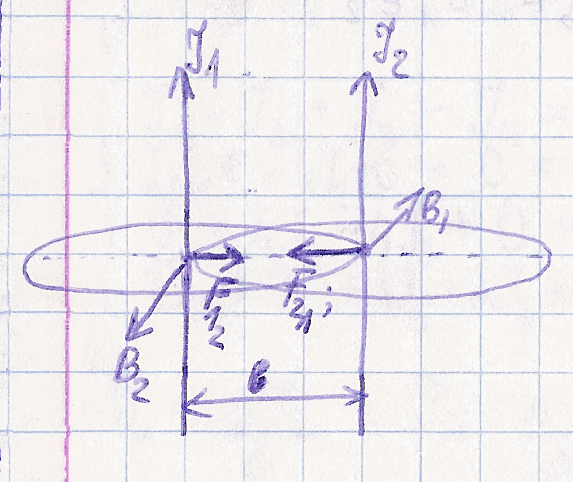
\includegraphics[height=0.5\textwidth]{images/bio_savaro_laplaso.png}
  \end{center}
  \caption{Bio-Savaro-Laplaso}
  \label{fig:bio_savaro_laplaso}
\end{figure}

\begin{defn}[Bio-Savaro-Laplaso dėsnis]
  Tarkime, kad turime du lygiagrečius begalinius laidininkus (žr.
  \ref{fig:bio_savaro_laplaso}), kuriais teka atitinkamai $I_{1}$
  ir $I_{2}$ stiprumo srovė, o tarp jų yra $b$ metrų tarpas.
  \begin{align*}
    \intertext{Tada pirmojo laidininko, antrojo laidininko taške,
    sukuriama indukcija bus lygi:}
    B_{1} &= \frac{\mu_{0}\mu 2 I_{1}}{4 \pi b} \\
    \intertext{Antrojo laidininko $dl$ ilgio atkarpą veiks jėga:}
    dF
    &= I_{2} \cdot B_{1} \cdot dl \\
    &= \frac{\mu_{0}\mu}{4 \pi} \frac{I_{1}\cdot I_{2}}{b} dl \\
  \end{align*}
  Gautoji išraiška vadinama Bio, Savaro, Laplaso dėsniu.
\end{defn}

TODO: Išsiaiškinti ir suprasti. (Fizika12.png)
TODO: Išsiaiškinti ir suprasti. (Fizika13.png)

\subsection{Atomų magnetiniai momentai}

Klasikinėje fizikoje apie branduolį skriejantį elektroną greičiu
$\vec{v}$ orbita, kurios spindulys yra $r$ apibūdina orbitinis judesio
kiekio momentas:
\begin{align*}
  \vec{L_{e}} &= \vec{r} \times m \vec{v} \\
\end{align*}
Elektrono orbitinė srovė:
\begin{align*}
  I
  &= e \nu \\
  &= \frac{e v}{w \pi r} \\
  &= \frac{e}{T} \\
\end{align*}
TODO: …
Elektrono orbitinis magnetinis momentas:
\begin{align*}
  \vec{p_{m}}
  &= I S \\
  &= \frac{e}{T} \pi r^{2} \\
  &= \frac{1}{2} e v r \\
\end{align*}
Vektorius $\vec{p_{m}}$ nukreiptas priešinga vektoriui $\vec{L_{e}}$
kryptimi. Vektorių $\vec{p_{m}}$ ir $\vec{L_{e}}$ modulių santykis
\begin{equation}
  \frac{p_{m}}{L_{e}} = \frac{e}{2m}
  \label{eq:giro_magnetinis_santykis}
\end{equation}
vadinamas giromagnetiniu santykiu. Atsižvelgę į
\ref{eq:giro_magnetinis_santykis} galima parašyti:
\begin{equation*}
  \vec{p_{m}} = - \frac{e}{2m} \vec{L_{e}}
\end{equation*}
Taigi su kiekvienu elektrono apie branduolį judėjimu yra susijęs tam
tikras orbitinis magnetinis momentas, apibūdinantis srovės magnetinį
lauką.

A. Einšteinas ir V. de Hasas 1915 metais parodė, kad be orbitinio
magnetinio momento, kiekvienas elektronas turi savąjį judesio
kiekio momentą $\vec{L_{S}}$, vadinamą sukiniu arba spinu, o su
juo susijęs savasis magnetinis momentas:
\begin{equation*}
  \vec{p_{ms}} = -\frac{e}{m} \vec{L_{s}}
\end{equation*}

Medžiagos struktūrinės dalelės (atomo, molekulės) atstojamasis
magnetinis momentas yra visų jos elektroninių orbitų ir savųjų
magnetinių geometrinė suma (pačio branduolio magnetinis 
momentas yra lygus 0, arba labai mažas ir čia į jį nėra atsižvelgiama).
\begin{equation*}
  \vec{p_{a}} = \sum _{i} \vec{p_{ml_{i}}} \sum _{j} \vec{p_{ms_{j}}}
\end{equation*}

Jeigu medžiagos atomo ar molekulės atstojamas magnetinis momentas
$\vec{p_{a}} \neq 0$, net tada, kai jų neveikia magnetinis laukas,
tokios medžiagos vadinamos paramagnetikais ($O_{2}, Al, Pt$).

Medžiagos, kurių $\vec{p_{a}} = 0$, vadinamos diamagnetikais.
(Intertinės dujos, daug organinių junginių, vanduo, stiklas,
Bi, Ag, An). Magnetiniame lauke diamegnetiko atomuose yra indukuojamas
magnetinis momentas.

Įmagnetėjimas:
\begin{align*}
  \vec{J}
  &= \frac{\vec{p}}{V} \\
  &= \frac{\sum_{i} \vec{p_{a_{i}}}}{V} \\
\end{align*}
čia:
\begin{description}
  \item[$\vec{p}$] – N skaičiaus dalelių magnetinių momentų geometrinė
    suma;
  \item[$V$] – tolygiai įelektrinto kūno makroskopinis tūris.
\end{description}
